% preamble
\documentclass[a4paper,12pt]{article}

\usepackage[ngerman]{babel}
\usepackage[utf8]{inputenc}
\usepackage{amsmath}
\usepackage{amsfonts}
\usepackage{hyperref}
\usepackage{graphicx}
\usepackage{minted}
\usepackage{float}
\usepackage{xcolor}

\setcounter{secnumdepth}{4}
\setcounter{tocdepth}{4}

% http://tex.stackexchange.com/questions/60209/how-to-add-an-extra-level-of-sections-with-headings-below-subsubsection


% body
\begin{document}

% Deckblatt
\begin{titlepage}
\title{Primzahlregression mit Hilfe genetischer Algorithmen}
\author{Björn Boss Henrichsen und Simon Budinsky\\Betreut von Herrn Christoph Fischer}
\date{\today}
\maketitle
\newpage
\end{titlepage}

\tableofcontents
\newpage

\section{Einleitung}
\subsection{Problemstellung}
In der Mathematik gibt es einige charakteristische Zahlen, die auf Grund der Komplexität ihrer Bestimmung eine besondere Anwendung finden. Eine solche Zahl stellen unter anderem Primzahlen dar. Unter einer Primzahl versteht man eine natürliche Zahl größer eins, welche nur durch sich selbst und eins teilbar ist. Somit ist die Mächtigkeit der Teilermenge einer Primzahl zwei.

Über 2000 Jahre lang konnte man keinen praktischen Nutzen aus dem Wissen über die Primzahlen ziehen. Dies änderte sich erst mit dem Aufkommen elektronischer Rechenmaschinen, bei denen die Primzahlen beispielsweise in der Kryptographie eine zentrale Rolle spielen.

Primzahlen sind hierfür deshalb so gut geeignet, weil es bisher keine Formel gibt, welche Primzahlen effizient berechenbar generiert. 
\subsection{Ziel des Projektes}
Das Ziel unseres Projektes besteht darin, eine Folge zu finden, die Primzahlen möglichst gut beschreibt. Dazu setzen wir einen genetischen Algorithmus ein, welcher zu vorgegebenen Datenpunkten eine Regressionsfunktion bestimmen soll. Diese Datenpunkte sollen Primzahlen sein, welche wir mit Hilfe einer optimierten Variante des Siebes des Eratosthenes erzeugen.

\newpage

\section{Relevanz von Primzahlen}
\subsection{RSA-Verschlüsselung} 
In der Kryptographie gibt es Algorithmen, welche auf der Primfaktorzerlegung basieren. Ein modernes Beispiel hierfür ist der asymmetrische Verschlüsselungsalgorithmus RSA. Da bisher offiziell keine effiziente Methode gefunden wurde, Primfaktorzerlegung zu betreiben, ist eine Verschlüsselung mit RSA sicher.

\subsubsection{Funktionsweise RSA}
$\varphi(n)$: Eulersche Phi-Funktion\\
$\varphi(n) := |\{a \in \mathbb{N}|1\leq a\leq n \land ggT(a,n) = 1\}|$

\begin{enumerate}
\item Nimm zwei (sehr, sehr große) Primzahlen $p$ und $q$
\item Bilde das RSA-Modul $N = p * q$
\item Bestimme $\varphi(N) = \varphi(p * q) = \varphi(p) * \varphi(q) = (p-1) * (q-1)$
\item Wähle eine Zahl $e$ mit $1 < e < \varphi(N)$ mit $ggT(e, \varphi(N)) = 1$
\item Bestimme $d$ mit $e*d \equiv 1$  $mod$ $\varphi(N)$
\end{enumerate}

\noindent Jetzt bilden $(e,N)$ den öffentlichen und $(d,N)$ den privaten Schlüssel.\\
Mit Hilfe des privaten Schlüssels lässt sich ein Klartext $T$ zum Geheimtext $G$ verschlüsseln:\\\\
\indent $G = T^e$ $mod$ $N$\\\\
\noindent Der Geheimtext lässt sich mit dem öffentlichen Schlüssel wieder entschlüsseln:\\\\
\indent $T = G^d$ $mod$ $N$\\

\subsubsection{Der RSA-Wettbewerb}
Aktuell gibt es einen \href{https://en.wikipedia.org/wiki/RSA_Factoring_Challenge}{RSA-Wettbewerb}. Ziel ist es, die zwei Primfaktoren $p$ und $q$ einer RSA Zahl $N$ zu finden. Denn findet man diese, so ist die Verschlüsselung geknackt. \\Dies wird mit einem entsprechenden Preisgeld belohnt.
Die bisher größte zerlgte RSA Zahl hat 232 Dezimalstellen (768 Bits, RSA-768) und wurde am 12. Dezember 2009 von Thorsten Kleinjung, Paul Zimmermann u.a. für ein Preisgeld von \$ 50000 USD faktorisiert. Hierfür wurde ein Rechencluster verwendet, welches etwa tausend Mal schneller als ein 2,2GHz AMD Opteron single-core Prozessor ist. Trotzdem dauerte die Faktorisierung zwei Jahre.\\ 
Dabei muss bedacht werden, dass heutzutage eher längere RSA-Zahlen verwendet werden. Häufig verbreitet sind Zahlen im Bereich von 309 bis 617 Dezimalstellen (1024-2048 Bits (das Preisgeld für eine RSA-2048-Zahl beträgt aktuell \$ 200000 USD (02.01.17))).

\subsubsection{Folgen einer geknackten Verschlüsselung}
Zusätzlich sollte die Verschlüsselung in ein paar Minuten, am besten wenigen Sekunden, erfolgen. So könnte das Passwort für den Bankaccount per Man-In-The-Middle-Angriff einfach ausgelesen werden. Dies ist natürlich nur eine von den vielen fatalen Folgen, wenn RSA geknackt werden würde. Der Mensch könnte seine Privatsphäre verlieren und zum ,,gläsernen Menschen“ werden.
\subsection{Primzahltests}
Eine primzahlbeschreibende Folge wird vor allem in der Kryptographie benötigt. Damit RSA funktioniert, werden zunächst zwei Primzahlen erzeugt. Diese müssen zunächst gefunden werden.\\ Hierfür werden Test wie der Rabin-Miller-Test verwendet, der allerdings nur über eine Zahl zwei Aussagen treffen kann: zusammengesetzt oder wahrscheinlich prim. \\Er liefert also nicht mit hundertprozentiger Sicherheit Zahlen, die anschließend für RSA verwendet werden. Ist eine Zahl nicht prim, funktioniert der RSA-Algorithmus nicht und kann geknackt werden. \\
Dies kann verhindert werden, indem stets mit hundertprozentiger Sicherheit über eine Zahl ausgesagt werden kann, ob sie prim ist. Hierfür könnte eine Folge für Primzahlen verwendet werden und somit die Primzahltest ablösen.
\subsection{Finden der $n$ten Primzahl}
Ein weiteres Problem ist folgendes: Finde die $n$te Primzahl.\\ Beim Sieb des Eratosthenes zum Beispiel müssen zunächst alle Primzahlen vor der $n$ten gefunden werden. Gäbe es eine Folge für Primzahlen, könnte dieses Problem wesentlich effizienter gelöst werden. Folglich wären Algorithmen zum Finden von Primzahlen wie das Sieb des Eratosthenes obsolet.

\subsection{Die größte Primzahl}
Vor etwa 2300 Jahren hat Euklid bewiesen: Es gibt unendlich viele Primzahlen. Dies wurde 1737 durch Leonhard Eulers Beweis bestärkt, der folgendes zeigte:\\\\
\indent $\sum_{p\in\mathbb{P}}{\frac{1}{p}} = \infty$\\

\noindent Heutzutage versucht man stets größere Primzahlen zu finden. Daraus wurde eine Art Wettbewerb.
Die Aktuell größte Primzahl (Stand Januar 2017)  hat 22.338.618 Dezimalstellen und wurde 2016 vom \emph{Great Internet Mersenne Prime Search}-Projekt gefunden.\\
Bei der Suche kann jeder teilnehmen. Hierfür muss lediglich eine kostenlose Software heruntergeladen werden, welche nach Primzahlen sucht. Findet der Comupter eine neue ,,größte" Primzahl, erhält man \$3000 USD.\\
Mit Hilfe einer Folge für Primzahlen könnte diese direkt gefunden werden.



\newpage{}


\section{Das Sieb des Eratosthenes}
\subsection{Allgemein}
Das Sieb des Eratosthenes ist ein Algorithmus, mit welchen man Primzahlen findet kann. \\Er wurde
nach dem griechischen Mathematiker Eratosthenes von Kyrene benannt, welcher im 3. Jahrhundert v. Chr. lebte. \\Laut \href{https://de.wikipedia.org/wiki/Sieb_des_Eratosthenes}{wikipedia.org} habe dieser selbst nicht das Verfahren entdeckt. Eratosthenes habe lediglich die Bezeichnung ,,Sieb“ eingeführt.\\
Für Primzahlen kleiner 10.000.000 zählt der Algorithmus zu den effizientesten Methoden. Für größere Zahlen empfehlen sich effizientere Algorithmen. Beispiele sind der Lehmann-Test oder der Rabin-Miller-Test, welcher auch in modernen Verschlüsselungsalgorithmen (RSA) verwendet wird.

\subsection{Funktionsweise}
Zu Beginn werden alle natürlichen Zahlen von 2 bis einer Grenze $n$ aufgeschrieben. Anfangs sind all diese nicht gestrichen und somit potentielle Primzahlen. Nun durchläuft man das Intervall. Trifft man auf eine ungestrichene Zahl, so ist diese eine Primzahl. Jetzt werden alle Vielfachen dieser gestrichen, die größer oder gleich deren Quadrat sind. Ist man am Ende des Intervalls angekommen, liegen sowohl gestrichene als ungestrichene Zahlen vor. Dabei ist jede ungestrichene Zahl prim.

Es genügt, die Vielfachen von Primzahlen zu streichen, die kleiner oder gleich der Wurzel der Grenze $n$ sind. Denn ist ein Primfaktor einer zusammengesetzten Zahl immer kleiner gleich der Wurzel der zusammengesetzten Zahl.

Außerdem muss beim Streichen der Vielfachen erst mit dem Quadrat der Primzahl begonnen werden, da alle kleineren Vielfachen bereits getrichen wurden.

\newpage{}

\subsection{Offizielle Variante}

\subsubsection{Programmablaufplan}
\begin{figure}[h]
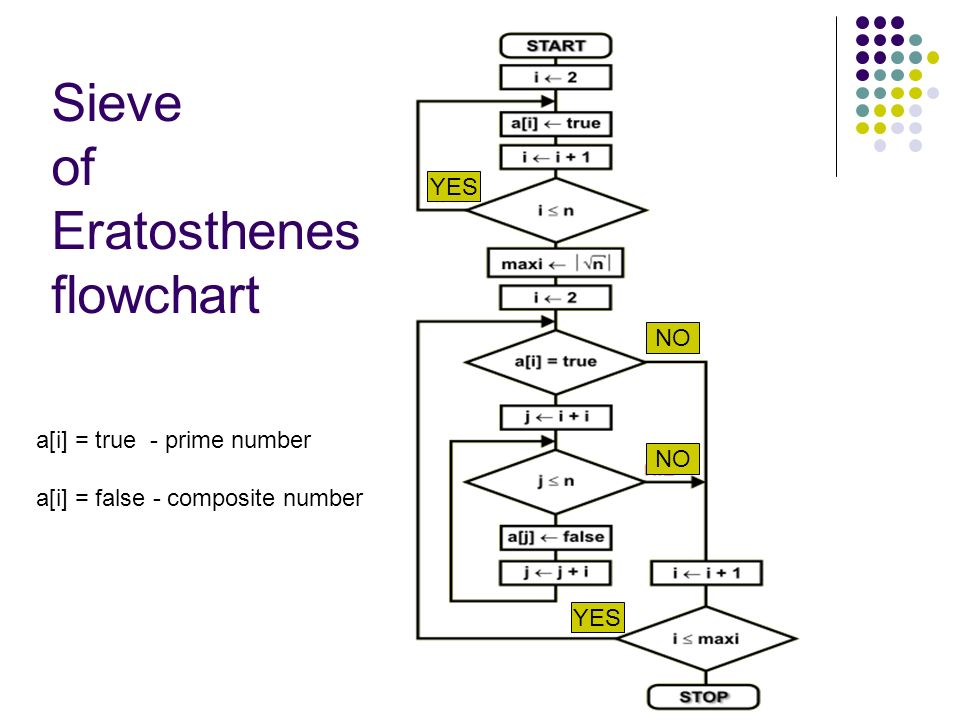
\includegraphics[width=\textwidth]{eratosthenesPAP.jpg}
\end{figure}

\subsubsection{Komplexität}
Die asymptotische Laufzeitkomplexität $O$ in Abhängigkeit von einer oberen Grenze $n$ ergibt sich wie folgt:\\\\
Sei $p_j \in \mathbb{P}$\\
So werden für jede Primzahl 
\[ p_j \leq \sqrt{n} \]
höchstens $\frac{n}{p_j}$ Zahlen gestrichen. Somit erhält man für die Anzahl an ,,Streichungen":\\
\[ \frac{n}{2} + \frac{n}{3} + \frac{n}{5} + ... = \sum_{p_j\leq\sqrt{n}}{\frac{n}{p_j}} = n * \sum_{p_j\leq\sqrt{n}}{\frac{1}{n}}\]
Nun muss die asymptotische Ordnung $O$ vom zweiten Faktor gefunden werden. Diese ist $O$(log log $n$) (Der Beweis hierfür ist nicht trivial und würde den Rahmen der Facharbeit sprengen). Daher ergibt sich eine Gesamtkomplexität von $O$($n$ log log $n$).


\subsection{Optimierungsmaßnamen}

\subsubsection{Weglassen der eins}
Da die eins keine Primzahl ist, kann man sie vorab ignorieren. Somit wird die Länge des primes-Puffers um ein Byte verringert (Speichereffizienz). Zusätzlich muss zu Beginn ein Byte weniger initialisiert werden. In der äußeren for()-Schleife wird ebenfalls ein Durchlauf weniger benötigt (Zeiteffizienz).\\

\subsubsection{Quadrieren statt Radizieren}
Des Weiteren ist das Quadrieren an einem Computer effizienter als das Radizieren. Dies erklärt sich darin, dass für das Radizieren eine Bisektion (Software) benötigt werden kann. Dahingegen ist das Quadrieren lediglich eine Multiplikation, welche direkt in der ALU (Hardware) ausgeführt wird.\\
Somit kann man schreiben:\\\\
$i$: Aktuell betrachtete Zahl\\
\[ i \leq \sqrt{n} \Rightarrow i * i \leq n \]

\subsubsection{Zahlen im Vorraus streichen}
Der Algorithmus kann weitergehend optimiert werden, indem man Zahlen vorab ,,streicht“. So haben wir alle Vielfachen von zwei bereits ,,gestrichen“. Daraus ergibt sich folgende Speichereinsparung:\\
\\
$a$: Belegter RAM-Speicher mit allen Zahlen [0;$n$]\\
$b$: Belegter RAM-Speicher ohne eins und geraden Zahlen\\
$n$: Obere Grenze des Siebes\\
$k$: Proportionalitätsfaktor\\

\begin{align}
a &= k * b\\
\Leftrightarrow n &= k * ( \frac{n}{2} - 1 )\\
\Leftrightarrow k &= \frac{n}{( \frac{n}{2} - 1 )}\\
&= \frac{2n}{n-2}
\end{align}
\\
Foglich verwendet die optimierte Variante $\frac{n-2}{2n}$ Mal so viel Speicher, im Vergleich zur offiziellen. Somit können mehr Primzahlen auf dem gleichen Rechner gefunden werden.\\
\\
Auch zeigen unsere Messungen, dass, wenn man alle Vielfachen von zwei weglässt, der Algorithmus mehr als doppelt so schnell terminiert (Zeiteffizienz).\\
\\
Nach den oben genannten Optimierungen könnte ein Programmablaufplan so aussehen:\\\\
\begin{figure}[H]
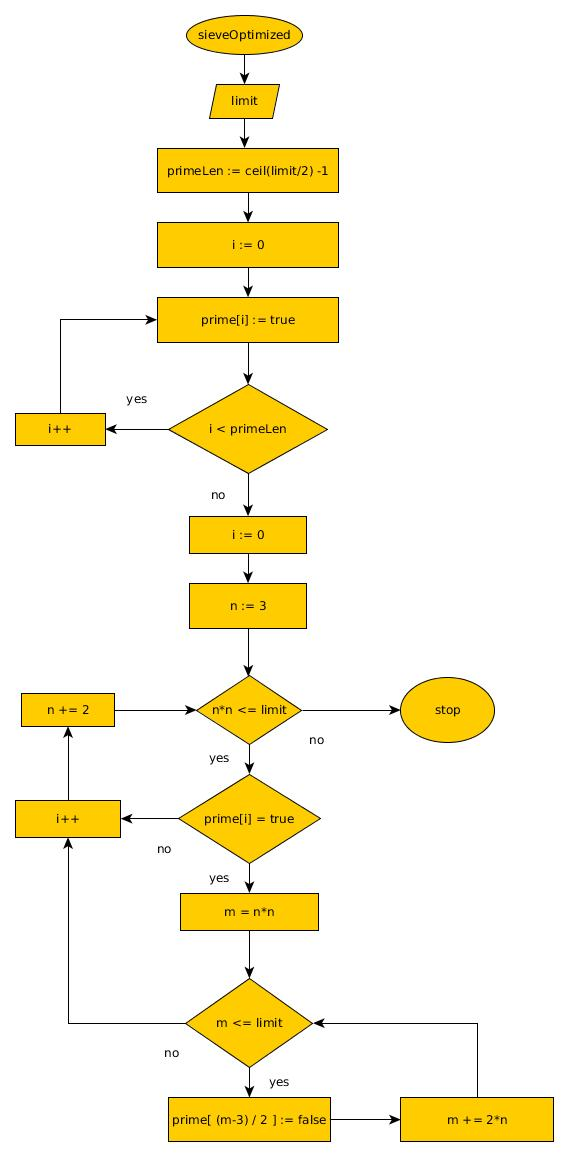
\includegraphics[width=\textwidth,height=\textheight,keepaspectratio]{sieveOptimized.jpg}
\end{figure}

\noindent Nun könnte man immer mehr Zahlen im Vorraus ,,streichen". Hierfür gibt es allerdings andere Algortihmen. Das \emph{Sieb des Atkin} zum Beispiel schließt vorher Zahlen bestimmter Restklassen aus und hat eine lineare Laufzeitkomplexität $O(n)$.

\subsection{Messungen}
\subsubsection{Methodik}
Um die Laufzeit des Siebes für verschiedene Grenzen $limit$ zu messen, wurde das Programm für jedes $limit$ jeweils neu kompiliert und ausgeführt. Nachdem die Primzahlen gefunden sind, gibt das Programm die böntigte Zeit zwischen Speicherallokation für den Primzahl-Puffer und dem Finden der Primzahlen in Sekunden aus. Diese Ausgabe wurde in eine .csv-Datei per Linux-Bash umgeleitet, um somit später mit LibreOfficeCalc Diagramme zu erzeugen. Dabei besteht diese Datei aus drei Spalten. Die erste Spalte repräsentiert die aktuelle Grenze $limit$, die zweite die gemessene Zeit in Sekunden und in der dritten Spalte steht die Anzahl gefundener Primzahlen.
\\\\
\noindent Dafür verwendeten wir folgendes Bash-Script:

\begin{minted}[linenos,frame=lines]{bash}
#!/bin/bash
#i: limit
for i in {100000000..6000000000..100000000}
do
    echo -n "$i," >> runtimes.csv
    gcc -std=c11 -DLIMIT=$i sieveRuntime.c -o sieveRuntime -lm \
		&& ./sieveRuntime >> runtimes.csv
done
\end{minted}

\noindent Wir implementierten folgende Algorithmen in C zur Zeitmessung:
\newpage
\noindent \textbf{Sieb ohne die eins:}
%\newpage
\begin{minted}[linenos,frame=lines]{C}
#include    <inttypes.h>
#include    <stdbool.h>
#include    <stdlib.h>
#include    <string.h>
#include    <sys/time.h>
#include    <stdio.h>

int main( void ) {
    struct timeval  start, end;
    gettimeofday(&start, NULL);
    
    bool* prime = (bool*)malloc(sizeof(bool) * (LIMIT-1));
    if( prime == NULL ) return 1;
    memset(prime, true, LIMIT-1);

    for(uint64_t i = 2; i*i <= LIMIT; i++) {
        if(prime[i-2]) {
            for(uint64_t j = i*i -2; j <= LIMIT; j += i)
                prime[j] = false;
	}
    }


    gettimeofday(&end, NULL);
    
    // Count primes
    uint32_t    nPrimes  = 0;
    for( uint32_t i = 0;  i < LIMIT-1; i++)
        if( prime[i] ) nPrimes++;
    
    printf("%.10f,%" PRIu32 "\n", 
	 end.tv_sec + end.tv_usec/1e6 - start.tv_sec - start.tv_usec/1e6, 
	  nPrimes);
    
	return 0;
}
\end{minted}

\newpage
\noindent \textbf{Sieb ohne die eins und geraden Zahlen:}
\begin{minted}[linenos,frame=lines]{C}
#include    <inttypes.h>
#include    <stdbool.h>
#include    <stdlib.h>
#include    <string.h>
#include    <sys/time.h>
#include    <stdio.h>
#include    <math.h>

int main( void ) {
    struct timeval  start, end;
    gettimeofday(&start, NULL);

    uint32_t primeLen = ceil(LIMIT / 2) - 1;
    bool*    prime    = (bool*)malloc(sizeof(bool) * primeLen);
    if( prime == NULL ) return 1;
	memset(prime, true, primeLen);

    for(uint64_t i = 0, n = 3;  n*n <= LIMIT;  i++, n += 2) {
        if(prime[i]) {
            for(uint64_t m = n*n;  m <= LIMIT;  m += 2*n)
			    prime[ (m-3) / 2 ] = false;
        }
    }

    gettimeofday(&end, NULL);
    
    // Count primes
    uint32_t    nPrimes  = 1;
    for( uint32_t i = 0;  i < primeLen; i++)
        if( prime[i] ) nPrimes++;
    
    printf("%.10f,%" PRIu32 "\n", 
     end.tv_sec + end.tv_usec/1e6 - start.tv_sec - start.tv_usec/1e6, 
      nPrimes);
      return 0;
}
\end{minted}
\newpage
\noindent \textit{[Anmerkung:]}\\
Es wird bewusst nicht die Zeit zum Ausgeben (printf()) mit einbezogen, da diese allgemein einen großen Anteil an Laufzeit beansprucht. So ergibt sich bei unserem optimierten Algorithmus für n = 1.000.000 eine Zeit von etwa 1389.054 Sekunden mit Ausgabe aller Primzahlen und etwa 8.0484920487 Sekunden ohne.\\\\

\noindent Die Messungen fanden in folgender Umgebung statt:\\\\
\begin{tabular}{|r|l|}
\hline
Operating System & \emph{Linux Mint 18.1 Cinnamon 64-Bit}\\
Cinnamon Version & \emph{3.2.7}\\
Linux Kernel & \emph{4.4.0-53-generic}\\
Processor & \emph{Intel Core i5-4440 CPU @ 3.10GHz x 4}\\
Memory RAM & \emph{7.7GiB}\\
\hline
\end{tabular}\\\\

\subsubsection{Vergleich zwischen offizieller und optimierter Variante}
$t_g$: Benötigte Zeit in Sekunden, offizielle Variante (blau)\\
$t_u$: Benötigte Zeit in Sekunden, optimierte Variante (rot)\\
\begin{tabular}{|c|c|c|c|}
\hline
$limit$ & $t_g$[s] & $t_u$[s] & $\frac{t_g}{t_u}$\\
\hline
100000000 & 1,6142570771 & 0,6927529358 & 2,3302060427\\
200000000 & 3,3796610065 & 1,5407490117 & 2,193518205\\
300000000 & 5,2564000593 & 2,2783710453 & 2,3070869296\\
400000000 & 6,7034089816 & 3,1714290402 & 2,1136872043\\
500000000 & 8,9381100896 & 3,9901179841 & 2,2400616035\\
600000000 & 10,3455499889 & 5,011878017 & 2,0642062624\\
700000000 & 12,6841129465 & 5,5832778916 & 2,271803982\\
800000000 & 13,9744109066 & 6,8093409411 & 2,0522413296\\
900000000 & 15,8358931078 & 7,3026679844 & 2,1685078853\\
1000000000 & 18,0069118877 & 8,0484920487 & 2,2373025629\\
1100000000 & 19,4879198822 & 9,4263940965 & 2,0673780114\\
1200000000 & 22,4203640433 & 10,0174689825 & 2,2381266248\\
1300000000 & 23,5954410898 & 10,3775840185 & 2,2736930915\\
1400000000 & 26,5114490883 & 11,0751651153 & 2,393774613\\
1500000000 & 26,9755919041 & 11,9925879208 & 2,2493553587\\
1600000000 & 30,2582220339 & 13,9449501191 & 2,1698336513\\
1700000000 & 32,2235829942 & 14,2521269333 & 2,2609666013\\
1800000000 & 32,8872118869 & 14,924550968 & 2,2035645801\\
1900000000 & 36,7206629502 & 16,3945279494 & 2,2398121534\\
2000000000 & 38,3611690887 & 16,617560026 & 2,3084718231\\
2100000000 & 39,3934800971 & 17,4123429244 & 2,2623882534\\
2200000000 & 42,4355878925 & 19,252283056 & 2,2041847073\\
2300000000 & 43,353328041 & 20,0979319791 & 2,1571039292\\
2400000000 & 45,0081739355 & 20,6734950301 & 2,1770955453\\
2500000000 & 49,1815101048 & 22,0877529756 & 2,2266416217\\
2600000000 & 51,3432890466 & 22,012063034 & 2,3325069062\\
2700000000 & 51,1586249138 & 24,0191830281 & 2,129906952\\
2800000000 & 53,3409920051 & 24,7522308979 & 2,1549973505\\
2900000000 & 55,47018401 & 24,3075119497 & 2,282018173\\
3000000000 & 56,9847639827 & 26,5199970692 & 2,148746994\\
3100000000 & 60,5142700262 & 27,7222269376 & 2,1828791086\\
3200000000 & 60,012045889 & 28,7487220151 & 2,0874683006\\
3300000000 & 65,3936210892 & 29,68840601 & 2,2026652784\\
3400000000 & 62,9704729115 & 29,7541698854 & 2,116357914\\
3500000000 & 69,8409569373 & 31,0977290192 & 2,2458539302\\
3600000000 & 67,1172831177 & 30,4034039054 & 2,2075581842\\
3700000000 & 73,4939509822 & 32,2375419811 & 2,2797628624\\
3800000000 & 76,0375679339 & 31,9458291063 & 2,3802033023\\
3900000000 & 78,455664996 & 33,7550660629 & 2,3242634113\\
4000000000 & 80,9324689933 & 35,4401829989 & 2,2836357531\\
4100000000 & 82,0384289596 & 37,5744409737 & 2,1833572725\\
4200000000 & 79,314230075 & 36,3971849106 & 2,1791308935\\
\hline
\end{tabular}

\begin{figure}
\includegraphics[width=\textwidth,height=\textheight,keepaspectratio]{comparison.png}
\end{figure}


\subsubsection{Messung mit Ausgabe aller Primzahlen}
\begin{tabular}{|c|c|c|c|c|}
\hline
$limit$ & $t_g$[s] & $t_u$[s] & $\Delta t$ & $anzahl$ \\
\hline
100.000 & 0,003 & 0,002 & 0,001 & 9592\\
1.000.000 & 1,216 & 1,205 & 0,011 & 78498\\
10.000.000 & 14,463 & 14,387 & 0,076 & 664579\\
100.000.000 & 143,18 & 142,439 & 0,741 & 5761455\\
1.000.000.000 & 1397,5 & 1389,054 & 8,446 & 50847534\\
\hline
\end{tabular}
\newpage

\section{Genetischer Algorithmus für Regressionen}
\subsection{Definition genetischer Algorithmus}
Ein genetischer Algorithmus, oder auch Evolutionärer Algorithmus, ist eine Klasse von Algorithmen, welche an die Funktionsweise der Natur angelehnt sind.\\
Hierbei werden aus einer Datenmenge, die dafür bestimmt ist, ein bestimmtes Problem zu lösen, die effizientesten ausgewählt und dafür verwendet die Anzahl an Datenmengen erneut zu erweitern mit  den effizientesten als Grundgerüst.\\ Somit „lernt“ der Algorithmus aus seinen Fehlern, da nur die effizientesten Datenmengen „überleben“. 

\subsection{Funktionsweise eines genetischen Algorithmus}
Zu Beginn wird erst einmal eine Darstellungsweise für das zu lösende Problem aufgestellt. \\
Anschließend wird eine Population generiert mit einer zufällig aufgebauten, oder bereits leicht geordneten, Struktur dieser Darstellungsweise. Anschließend muss jedes Element dieser Population von einer bewertenden Funktion, meist der Fitness-Funktion, die Fitness des Elements berechnen/bewerten. \\
Diese Funktion ist notwendig da es sonst, wie in der Natur auch, keinen Grund gäbe sich zu verändern, wenn es nicht für das Überleben beziehungsweise das Wohlergehen notwendig ist. Die Fitness-Funktion wird basierend auf das Problem festgelegt und ist in ihrer Struktur meistens einfacher. So kann diese beispielsweise bei einem Algorithmus, welcher ein simuliertes Auto zu fahren lernen soll, einfach nur eine Division von der zurückgelegten Strecke durch die benötigte Zeit sein. \\
Nachdem jedes Element der Population bewertet wurde und jedem ein Fitness Wert zugeordnet worden ist müssen die Elemente die am besten abgeschnitten haben aussortiert werden. In unserem Beispiel von oben wären dies die Elemente, welche die höchste Fitness erreicht haben. Dies ist aber nicht zwingend. So kann es auch sein, dass eine kleinere Fitness besser, als eine größere ist. Das hängt von der Fitness-Funktion und deren Funktionsweise ab. \\
Diese besseren ausgewählten Elemente repräsentieren nun die Eltern. Diese werden nun aus der Population entfernt und außerhalb gespeichert. Anschließend werden alle Elemente der Population gelöscht. \\
Nun wird für jeden Platz in der Population durch Zufall n, vorher festgelegte, Eltern aus den beiseitegelegten Elementen ausgewählt. Von diesen n Eltern werden nun, meist ebenfalls durch Zufall, Teile aus der Datenmenge entnommen und in das neue leere Element der Population getan. \\
Anschließend kann es noch zu einer geringen Wahrscheinlichkeit, die meist als 1 bis 2 Prozent angelegt ist, zu einer Mutation kommen. Diese Mutation ist notwendig, damit sich die Population nicht auf den am Anfang durch Zufall erstellten Datenmengen festfährt, sondern immer was Neues hinzukommt und was Altes entfernt wird. Anschließend können die beiseitegelegten Elemente ebenfalls entfernt werden, da man für diese keinen Nutzen mehr hat. \\
Nun kann der gesamte Prozess von vorne beginnen mit der neu erstellten Population, die auf der alten Population aufbaut und die statistisch betrachtet nun bessere Fitness Werte erzielen wird. 

\begin{figure}[H]
\includegraphics[width=\textwidth,height=\textheight,keepaspectratio]{Flowchart_Gen_Alg.png}
\end{figure}

\subsection{Unsere Implementierung}
\subsubsection{Die Funktionssyntax}
Damit der Algorithmus mit mathematischen Funktionen umgehen kann, bedarf es einer speziellen Funktionssyntax, welche von diesem interpretiert werden muss.\\
Wir haben uns für eine Assembler-Artige Darstellung von mathematischen Funktionen entschieden, wobei ein ,,Term" wie folgt aufgebaut ist:
\indent \begin{center}
$Funktion$ $Parameter_a$ optional $Parameter_b$ $Solution$\\
\end{center}
Dabei repräsentieren konstante Bytes mathematische Funktionen, um den Speicherverbrauch möglichst gering zu halten (im Vergleich zur Verwendung von Zeichenketten):

\begin{minted}[linenos,frame=lines]{C}
VAR  = 0x00, //Usage of Variable x
SLA  = 0x01, //Temp. Solution A
SLB  = 0x02, //Temp. Solution B
NUM  = 0x03, //following is a double
ADD  = 0x10, //double add(double a, double b)       -> a + b
SUB  = 0x11, //double substract(double a, double b) -> a - b
MUL  = 0x12, //double multiply(double a, double b)  -> a * b
DIV  = 0x13, //double divide(double a, double b)    -> a / b
POW  = 0x14, //double power(double a, double b)     -> a ^ b
LOG  = 0x15, //double logarithm(double a, double b) -> log(a) / log(b)
RND  = 0x16, //double round(double a)               -> (int64_t)(a + 0.5)
ABS  = 0x17, //double absolute(double a)            -> +a
SIN  = 0x18, //double sin(double a)                 -> sin(a)
COS  = 0x19, //double cos(double a)                 -> cos(a)
TAN  = 0x1a, //double tan(double a)                 -> tan(a)
ASIN = 0x1b, //double arcsin(double a)              -> asin(a)
ACOS = 0x1c, //double arccos(double a)              -> acos(a)
ATAN = 0x1d, //double arctan(double a)              -> atan(a)
EXP  = 0x1e, //double exponent(double a)            -> e ^ a
RET  = 0xff  //end of function
\end{minted}
\newpage

\paragraph{Beispiel}
\[(|sin(x) + cos(x)|)^{tan(6)}\]\\

\noindent Dies sieht schließlich wie folgt aus:

\noindent 
\begin{center}
\textit{
SIN VAR SLA\\ COS VAR SLB \\
ADD SLA SLB SLA\\
ABS SLA SLA\\
TAN NUM 6.0 SLB\\
POW SLA SLB SLA\\
RET SLA
}
\end{center}

\noindent \\ Das würde folgendes bewirken:\\
Zuerst wird der Sinus von der Variable berechnet und im temporären Register A gespeichert.\\
Anschließend wird der Cosinus der unabhängigen Variable berechnet und im temporären Register B gespeichert.\\
Die Werte dieser Register werden nun miteinander addiert und wieder im Register A gespeichert. \\
Von dem Wert in Register A wird nun der Betrag genommen und wieder in Register A zurückgespeichert. \\
Nun wird der Tangens der Dezimalzahl 6.0 berechnet und in Register B gespeichert. \\
Danach wird der Wert von Register A hoch den Wert von Register B gerechnet und dies im Register A gespeichert. \\
Zum Schluss wird Register A als das mit dem Ergebnis anerkannt und die Funktion wird beendet. 

\newpage
\subsubsection{Definitionen}
\paragraph{Headerdatei primereg.h}

\begin{minted}[linenos,frame=lines,breaklines=true]{C}
#pragma once

#define N_FUNCTIONS         256  //Number of Functions per generation
#define N_PARENTS           32   //Number of parents to pick
#define N_NUMBERS           32   //Number of Numbers needed
#define N_PRINTDATA         256  //Number of loops till print of data
#define PERC_MUTATION       5    //Chance in percent of a mutation of a function
#define PERC_INHERIT        60   //Chance of child taking over data from parent B
#define FUNCTION_START      0x10 //Number of first function
#define FUNCTION_ONEARG     0x16 //Number of first function to take one argument
#define FUNCTION_END        0x1e //Number of last function
#define MAX_RAND_DOUBLE     512  //Maximum double to be picked as random number
#define MAX_RAND_DOUBLE_DIG 5    //Digits of MAX_RANDOM_DOUBLE
#define PERC_ADD_NEW        60   //Percentage of adding a new function on creation

#define DEBUG                    //If defined, every generation results will be printed to stdout
#ifdef  DEBUG
#undef  N_PRINTDATA
#define N_PRINTDATA 1
#endif // DEBUG
\end{minted}
\newpage
\paragraph{Erläuterung}\hfill\\\\
Diese stellen alle wichtigen Variablen des Quellcodes dar und können somit leicht verändert werden.\\ Hierbei Steht das N\_ für eine Nummer/Anzahl, das PERC\_ für ein Prozentwert und die anderen für vordefinierte Werte. \\
Falls DEBUG definiert ist, dann werden alle Funktionen nach einem Loop ausgegeben. Sonst werden sie nur alle N\_PRINTDATA Durchläufe ausgegeben. \\

\noindent N\_FUNCTIONS gibt an, wie viele Elemente in unserer Population sein sollen.\\
N\_PARENTS gibt an, wie viele der besten Elemente in der Population erhalten bleiben sollen und als die Grundgerüste der neuen Elemente gewertet werden sollen.\\
N\_NUMBERS hält die Anzahl an Nummern, mit denen die der Elemente abgeglichen werden sollen. \\
N\_PRINTDATA gibt an, nach wie vielen Durchläufen des primären Loops die Daten ausgegeben werden sollen. \\
PERC\_MUTATION ist ein Prozentwert, der die Wahrscheinlichkeit einer Mutation des Elementes angibt. Dieser Wert sollte gering gehalten werden, da es sonst sehr schnell zu dem Fall kommen kann, dass die neuen Elemente keine Ähnlichkeit zu den N\_PARENTS Elementen mehr haben. \\
PERC\_INHERIT ist ein Prozentwert, der angibt, wie groß die Wahrscheinlichkeit ist, dass ein neues Element die Eigenschaft eines der besseren Elemente erbt. Dieser Wert sollte nicht zu groß werden, da die neuen Elemente sonst sehr schnell größer und komplexer werden, da sie dann nahezu alles ihrer Eltern übernehmen werden. \\
FUNCTION\_START gibt den Wert der ersten Funktion in unserem Syntax an.\\
FUNCTION\_ONEARG gibt den Wert der ersten Funktion an, die nur ein Argument und nicht zwei nimmt. \\
FUNCTION\_END gibt den Wert der letzten Funktion in unserem Syntax an.\\
MAX\_RAND\_DOUBLE stellt die maximale Größe eines durch Zufall generierten Zahlenwertes dar.\\
MAX\_RAND\_DOUBLE\_DIG stellt die maximale Anzahl an Nachkommastellen der durch Zufall generierten Zahlenwerte dar. \\
PERC\_ADD\_NEW gibt in Prozent an, wie groß die Wahrscheinlichkeit ist, dass eine Funktion bei der Initialisierung eine weitere mathematische Funktion erhält. (Alle erhalten mindestens eine)\\

\subsubsection{Wahl des Funktionsparameter Datentyps}
Wir haben uns dazu entschieden, den Datentypen double als den primären Datentypen für unsere Funktionen zu wählen, da dieser eine hohe Präzision gewährleistet, jeder x86 und x86-64 Prozessor mit diesem umgehen kann und er nur 8 Byte pro Variable aufnimmt. Zudem stellt die Mathematik-Bibliothek, welche wir für die mathematischen Funktionen verwendet haben, Funktionen bereit, welche mit double arbeiten. 

\subsubsection{Funktionsweise}
\paragraph{Programmablaufplan}
\begin{figure}
\includegraphics[width=\textwidth,height=\textheight,keepaspectratio]{Flowchart_Unser_Alg.png}
\end{figure}
\newpage

\paragraph{Erläuterung}\hfill\\\\
Unser Algorithmus startet damit, den Speicher für die Population zu allokieren. Anschließend allokiert er den Speicher für die Primzahlen, deren Erzeugung noch beschrieben wird. Danach wird der Zufallsgenerator mit der vergangenen Zeit seit dem 1. Januar 1970 in Millisekunden geseedet, damit wir möglichst zufällige Ergebnisse erhalten. \\

\noindent Nun werden die einzelnen Elemente der Population initialisiert. Hierfür wird die erste mathematische Funktion durch Zufall gewählt und deren Parameter ebenfalls als entweder VAR oder NUM. Anschließend wird geschaut, ob rand() mod 101 <= PERC\_ADD\_NEW gilt (Mit rand() mod 101 erhält man einen Zufallswert zwischen 0 und 100).  Wenn dies gilt, dann wird eine weitere zufällige mathematische Funktion hinzugefügt. Falls nicht, dann wird geschaut, ob beide Register einen Wert beinhalten. Falls ja, dann wird noch eine zufällige Funktion, die zwei Argumente nimmt, gewählt und die nimmt dann als Parameter die beiden Register. Somit ist gewährleistet, dass kein Wert verloren geht und man nur noch ein volles Register am Ende hat, welches dann als das mit dem Ergebnis gewählt wird. \\

\noindent Falls als Parameter NUM gewählt wird, so heißt das, dass eine zufällige Fließkommazahl generiert werden muss. Diese wird wie folgt erzeugt:\\
\noindent Zuerst wird ein HighDouble Wert erzeugt. Dieser liegt innerhalb der Grenzen 0 und MAX\_RAND\_DOUBLE. Anschließend wird ein LowDouble Wert erzeugt, welcher in den Grenzen 0 und 10\^MAX\_RAND\_DOUBLE\_DIG liegt. Dieser wird nun solange in einer Schleife durch 10 geteilt, bis er kleiner als 1 ist. Der Generierte Wert setzt sich dann zusammen aus dem HighDouble und dem LowDouble, die miteinander addiert werden. Zum Schluss wird noch geschaut, ob der Wert negativ sein soll, was durch ein Aufruf der rand() Funktion geschieht. \\

\noindent Als Beispiel:\\
MAX\_RAND\_DOUBLE 512\\
MAX\_RAND\_DOUBLE\_DIG 5\\
So werden als Zufallszahlen Zahlen zwischen -511.9999 und 511.9999 erzeugt. \\

\noindent Nachdem die gesamte Population mit validen Funktionen gefüllt worden ist, geht es in die Haupt-Schleife (\emph{Main-Loop}). Hier wird zum einen die evolve Funktion aufgerufen, welche im Grunde den genetischen Algorithmus beinhaltet, und dann wird noch eine Zählervariable gehalten, welche angibt, wann die Daten alle ausgegeben werden sollen, und eine, die die derzeitige Generation mit sich trägt.\\

\noindent In der evolve Funktion wird zuerst die Güte (\emph{Fitness}) der einzelnen Elemente der Funktion berechnet. Dabei wird diese anhand der Summe der Fehlerquadrate ermittelt: Diese Fitnessfunktion berechnet erst den Funktionswert des Elements für einen gegebenen x-Wert und anschließend seine Abweichung von der tatsächlichen Primzahl und quadriert diesen Wert. Diese Ergebnisse werden dann von x = 0 bis x = N\_NUMBERS - 1 berechnet und aufaddiert. Der dann erhaltene Wert repräsentiert die Fitness. Umso geringer dieser Wert ist, desto besser ist die Funktion.\\ \noindent Wichtig ist, dass wir mathematische Fehler als vollständigen Eliminierungsfaktor ansehen. So werden Funktionen, die beispielsweise versuchen durch 0 zu teilen, mit dem Fitnesswert -1.0 versehen, was sie als nicht gültig kennzeichnet. \\

\noindent Sobald die Fitness für jede Funktion berechnet wurde, werden nun die \\N\_PARENTS besten Elemente ausgewählt. Dies erfolgt mit Hilfe des Bubblesort Algorithmus, welcher dafür sorgt, dass die besten N\_PARENTS Elemente die ersten der Population sein werden. 
Wir haben uns dafür entschieden, die N\_PARENTS besten Elemente nicht für die neue Population zu verwerfen, da wir der Ansicht waren, dass es besser wäre, diese zu behalten. Somit werden in jedem Durchlauf lediglich N\_FUNCTIONS – N\_PARENTS Elemente der Population als neue Elemente aus den N\_PARENTS Elementen generiert. Dies hat ebenfalls zur Folge, dass eine Funktion, die die Fitness 0 hat und somit perfekt ist, nicht durch Zufall verändert wird, zum Schlechteren und dann rausgeworfen wird. Dadurch ist gewährleistet, dass die N\_PARENTS ersten Elemente der Population immer gute Werte erzielen werden. 

\noindent Anschließend wird der Zufallsgenerator erneut geseedet, da es in dem von uns gewählten eine gewisse Wiederholung nach ungefähr 10\^5 Zahlen gibt, die wir verhindern möchten (es werden keine \emph{true random numbers} erzeugt). Dann kommt es zur Neubildung der Population. Hierfür werden immer zwei der N\_PARENTS gewählt. Es kann auch vorkommen, dass diese beiden gleich sind. Das wirkt sich aber nicht negativ auf den Algorithmus aus und kann somit enthalten bleiben. 

\noindent Die \emph{repopulate}-Funktion ist die Zeitaufwändigste Funktion und zugleich die komplexeste. Zuerst geht sie durch die Funktion der Eltern und zählt alle mathematischen Funktionen, die in diesen aufgerufen werden. Anschließend allokiert sie genug Speicher, um einen Array von allen mathematischen Funktionen und deren Parametern zu erstellen, die bei den Eltern vorkommen. Nachdem sie diese mathematischen Funktionen der Eltern alle eingelesen hat, mutiert sie diese. Dies geschieht, indem die Funktion durch den Array geht und, sobald rand() mod 101 <= PERC\_MUTATION gilt, ersetzt sie entweder die mathematische Funktion oder einen der Parameter. Nachdem dieser Schritt getan ist, findet die Funktion ein verwendbares Erst-Element, dass keine Register als Parameter nimmt. Falls es keine mathematische Funktion findet, auf die dies zutrifft, verändert sie das erste Element des Arrays so, dass dieses keine abhängigen Parameter mehr nimmt. Zum Schluss geht es durch den Array von Funktionen und schaut, ob rand() mod 101 <= PER\_INHERIT gilt. Wenn dies der Fall ist, erbt das neue Element diese Mathematische Funktion von denen der Eltern, falls dies von den Parametern her zutrifft. Sie kann aber nicht vererbt werden, wenn die neue mathematische Funktion als Parameter Register A nimmt und Register B, aber Register A zu diesem Zeitpunkt leer ist. Dann wird diese Funktion übersprungen. Nach Durchgehen des Arrays wird, wie bei der Initialisierung, geschaut, ob in beiden Registern ein Wert ist und falls ja, dann wird erneut eine mathematische Funktion zufällig ausgewählt, die beide Parameter nimmt und nur ein Register zurückgibt. Zum Schluss wird noch der Schluss, also RET, an die Funktion angehangen und der reservierte Speicher wird freigegeben beziehungsweise der von dem neuen Element verkleinert. \\

\noindent Diese Funktion wird nun für jedes Element der Population ausgeführt, bis die gesamte Population erneut gefüllt wurde. Dann beginnt die Schleife wieder von vorne und die Fitness der neuen Funktionen wird erneut berechnet. \\
\newpage 

\subsection{Vor-/Nachteile gegenüber herkömmlichen Regressionsmethoden}
\subsubsection{Vorteile}
Da unser Algorithmus lediglich die neu erstellten Funktionen mit denen der eingegebenen Funktionen abgleicht, ist er dazu in der Lage, eine Regression für jegliche Funktionstypen durchzuführen, sofern man ihm die richtigen Funktionswerte zum Vergleichen gibt. So kann der Algorithmus beispielsweise ohne Vorwissen über den möglichen Funktionstyp eine lineare oder quadratische oder exponentielle Funktion finden. In unserem Beispiel füllen wir den Array mit Primzahlen, um eine Funktion zu finden, welche diese beschreibt. Wir haben ihn aber auch mit den Zahlen einer quadratischen Funktion gestartet, welche er innerhalb von 3 Generationen, also 3 Aufrufen der \emph{evolve}-Funktion, erfolgreich fand. \\

\subsubsection{Nachteile}
Der Speicherverbrauch und die Laufzeit lassen sich nicht einschätzen, da diese beiden Werte abhängig sind von der Rückgabe der rand() Funktion. Aber es lässt sich sagen, dass der Algorithmus für höhere N\_FUNCTIONS oder höhere N\_PARENTS mehr Zeit in Anspruch nehmen wird. Des Weiteren wird der Speicherverbrauch für höhere PERC\_ADD\_NEW und PERC\_INHERIT ebenfalls schneller ansteigen. Da für höhere PERC\_INHERIT die Tendenz des Speicherverbrauchs schnell steigend ist, muss man mit diesem Wert vorsichtig umgehen, da es sonst sehr schnell zu einem Speicherüberlauf kommen kann.\\
Auch liefert der Algorithmus keine Folge eines vorgegebenen Grades (wie etwa bei einer linearen, quadratischen, ... Regression), was für manche Sachverhalte unerwünscht sein kann.
\newpage

\section{Ergebnisse}
Um Folgen einer ausreichenden Güte zu erhalten, muss der Algorithmus über längere Zeit laufen. Im Rahmen der Arbeitsprojektwoche stand uns leider nur sehr wenig Zeit zur Verfügung. Trotzdem möchten wir einige Durchläufe dokumentieren.\\
\begin{figure}
\includegraphics[width=\textwidth,height=\textheight,keepaspectratio]{alg_list.png}
\end{figure}
\newpage

\section{Fazit}
Unser Algorithmus ist flexibel. Er versucht, alle ihm gegebene Datenpunkte möglichst gut zu approximieren, unabhängig davon, welchem Wachstum diese entstammen.\\
\noindent Allerdings muss man stets Glück haben, eine passende Folge zu finden. Dies ist darin zu begründen, dass diese per Zufall generiert werden. Somit ist das Verhalten des Algorithmus nicht vorhersehbar, weswegen konventienelle Regressionsmethoden schneller zu einem Ergebnis kommen.\\
\noindent Aber vielleicht hilft genau dieses Prinzip genetischer Algorithmen, Folgen für bisher unbekannte Wachstumsklassen, wie etwa Primzahlen, zu finden. Unsere bisherigen Messungen zeigen, dass unser Programm während der Laufzeit immer bessere Funktionen generiert. Somit könnte der Algorithmus irgendwann eine Folge für Primzahlen finden. Hierfür benötigen wir aber mehr Zeit und Rechenleistung.\\
\noindent Zusammenfassend konnte das volle Potential des Algorithmus im Rahmen der Arbeitsprojektwoche nicht völlig ausgeschöpft werden. Daher können wir zum aktuellen Zeitpunkt keine endgültige Aussage über die Eignung eines genetischen Algorithmus zur Regression treffen. Deshalb werden wir den Algorithmus weitergehend ausführen und sind auf dessen Ergebnisse gespannt.
\newpage

\begin{appendix}
\section{Quellen}
- https://en.wikipedia.org/wiki/Formula\_for\_primes\\
- https://de.wikipedia.org/wiki/Sieb\_des\_Eratosthenes\\
- https://de.wikipedia.org/wiki/Primzahl\\
- https://www.youtube.com/watch?v=ITLjfRiAc10\\
- http://www.iti.fh-flensburg.de/lang/algorithmen/asymp.htm\\
- http://www.programming-algorithms.net/article/41297/Sieve-of-Eratosthenes\\
- https://de.wikipedia.org/wiki/Miller-Rabin-Test\\
- http://www-cs-students.stanford.edu/\textasciitilde jl/Essays/ga.html\\
- https://en.wikipedia.org/wiki/RSA\_numbers\#RSA-768\\
- https://en.wikipedia.org/wiki/RSA\_Factoring\_Challenge\\
- https://de.wikipedia.org/wiki/Eulersche\_Phi-Funktion\\
- https://www.youtube.com/watch?v=oXlY-yx1oIw\\
- https://en.wikipedia.org/wiki/Sieve\_of\_Atkin\\
- https://en.wikipedia.org/wiki/Largest\_known\_prime\_number\\
- https://en.wikipedia.org/wiki/Divergence\_of\_the\_sum\_of\_the\_reciprocals\_of\_the\_primes\\
- https://de.wikipedia.org/wiki/Evolution\%C3\%A4rer\_Algorithmus\\
- THE NATURE OF CODE by Daniel Shiffman\\
\end{appendix}

\end{document}
